\documentclass{article}
\usepackage{amsmath}
\usepackage{graphicx}
\usepackage{float}
\usepackage{hyperref}
\usepackage{fancyvrb}
\usepackage{matlab-prettifier}

\setlength{\parindent}{0pt}

\title{CS663: Digital Image Processing - Homework 1}
\author{Harsh $\vert$ Pranav $\vert$ Swayam} 

\begin{document}

\maketitle
\section{Homework 1 - Question 1}

In this question, we are given two images of the same scene, but with different pixel sizes. But, for image alignment purposee, the size of the pixels should not be of importance, since transformation would depend on the pixel coordinates. Thus, image size should not affect the alignment process.

The original pixel size of the first image is $0.5 \times 0.5$, both sizes in mm.

\vspace{10pt}
For the first case, when the second image has a pixel size of $0.25 \times 0.25$, the new coordinates, which we represent as $(x', y')$, can be obtained from the original coordinates $(x, y)$ as follows:

\begin{equation}
\begin{bmatrix}
x' \\
y' 
\end{bmatrix}
=
\begin{bmatrix}
0.5 & 0 \\
0 & 0.5 \\
\end{bmatrix}
\begin{bmatrix}
x \\
y 
\end{bmatrix}
\end{equation}

Thus, the motion model that we can adopt to attain the desired alignment is the rigid (rotation + translation) model which will be followed by a scaling transformation in both X and Y directions based on the matrix given above.

\hrulefill
\vspace{5pt}

For the second case, when the second image has a pixel size of $0.25 \times 0.5$, the new coordinates, which we represent as $(x_2', y_2')$, can be obtained from the original coordinates $(x, y)$ as follows:

\begin{equation}
\begin{bmatrix}
x_2' \\
y_2'
\end{bmatrix}
=
\begin{bmatrix}
0.5 & 0 \\
0 & 1 \\
\end{bmatrix}
\begin{bmatrix}
x \\
y
\end{bmatrix}
\end{equation}

Thus, the motion model that we can adopt to attain the desired alignment is the rigid (rotation + translation) model which will be followed by a scaling transformation in {\bf only the X} direction based on the matrix given above.

\newpage
\section{Homework 1 - Question 2}


\subsection*{Given:}

$u_{12}$ represents the motion from $I_1$ to $I_2$ and a similar relation for $u_{23}$ and $u_{13}$.

\subsection*{Relation:}
$$u_{13}=u_{12}+u_{23}$$


\subsubsection*{Explanation:} 

Since the motion is solely transnational therefore the total displacement from $I_1$ to $I_3$ should be the sum of the displacement between $I_1$-$I_2$ and $I_2$-$I_3$.


\subsection*{Practicality:}


Some troubles may arise when this relations is used in practical. The reasons may be:


\subsubsection*{Numerical Approximations:} 

Numerical methods used in computation introduce rounding errors, which can accumulate and cause the computed motion vectors to deviate slightly from the theoretical relationship.


\subsubsection*{Noise:} 

The camera and other similar devices may be cursed with random noise, which can distort and hamper some features leading to small errors.

\newpage
\section{Homework 1 - Question 3}

From MATLAB and the graph, we have the following coordinates of the points in the image:
\begin{table}[H]
\centering
\begin{tabular}{|c|c|c|}
\hline
Sr. No. & Coordinates\_MATLAB & Coordinates\_Graph \\
\hline
1 & (242, 1520) & (-20, 635) \\
\hline
2 & (242, 50) & (-20, 543) \\
\hline
3 & (568, 422) & (0, 565) \\
\hline
4 & (568, 1142) & (0, 610) \\
\hline
\end{tabular}
\end{table}

Let us denote the graph coordinates as $(x_g, y_g)_i$ and the MATLAB coordinates as $(x_m, y_m)_i$ where $i$ is from 1 to 4.

\vspace{5pt}
From observing these points, we can see that the difference of $x_m$ (or $y_m$) coordinates gets scaled down by $\approx 0.0625 = \frac{1}{16}$ to give the $x_g$ (or $y_g$) coordinates.

\hrulefill

\vspace{5pt}
In {\bf mathematical representation}, we can write this as:
\begin{equation}
x_g = \frac{x_m}{16} + c_1
\end{equation}
\begin{equation}
y_g = \frac{y_m}{16} + c_2
\end{equation}
where $c_1$ and $c_2$ are constants that act as offsets such that the differences in the coordinates are preserved.

\hrulefill

\vspace{5pt}
In \textbf{matrix form}, we can write this as:
\begin{equation}
\begin{bmatrix}
x_g \\
y_g \\
1
\end{bmatrix}
=
\begin{bmatrix}
\frac{1}{16} & 0 & c_1 \\
0 & \frac{1}{16} & c_2 \\
0 & 0 & 1
\end{bmatrix}
\begin{bmatrix}
x_m \\
y_m \\
1
\end{bmatrix}
\end{equation}

For the points in consideration, we can calculate the values of $c_1$ and $c_2$, which come out to be $\approx-35.5$ and $\approx538.625$ respectively. The exact values cannot be calculated as the points are collected through manual inspection and are not exact.

\subsection*{Summary:} 
The coordinates of the points in the MATLAB image can be transformed to the coordinates in the graph image using the affine transformation matrix:
\begin{equation*}
A = \begin{bmatrix}
\frac{1}{16} & 0 & -35.5 \\
0 & \frac{1}{16} & 538.625 \\
0 & 0 & 1
\end{bmatrix}
\end{equation*}

\newpage
\section{Homework 1 - Question 4}

To perform motion estimation using control points for the given motion model, we need to estimate the unknown constants \(a, b, c, d, e, f, A, B, C, D, E, F\).

\subsection*{Given}
The motion models:
\[
x_2 = ax_1^2 + by_1^2 + cx_1y_1 + dx_1 + ey_1 + f
\]
\[
y_2 = Ax_1^2 + By_1^2 + Cx_1y_1 + Dx_1 + Ey_1 + F
\]
Here, \( (x_1, y_1) \) are the coordinates of a point in the first image, and \( (x_2, y_2) \) are the coordinates of the corresponding point in the second image. The goal is to estimate the coefficients \( a, b, c, d, e, f, A, B, C, D, E, F \) using a set of known control points.

\subsection*{System of Equations}
Suppose we have \(N\) control points, where each control point in Image 1 is denoted as \( (x_{1i}, y_{1i}) \) and the corresponding point in Image 2 as \( (x_{2i}, y_{2i}) \) for \( i = 1, 2, \ldots, N \).

For each control point, we have two equations:

\[
x_{2i} = a x_{1i}^2 + b y_{1i}^2 + c x_{1i}y_{1i} + d x_{1i} + e y_{1i} + f
\]
\[
y_{2i} = A x_{1i}^2 + B y_{1i}^2 + C x_{1i}y_{1i} + D x_{1i} + E y_{1i} + F
\]

\subsection*{Matrix Form}
For the \(x_2\) coordinate:
\[
\begin{bmatrix}
x_{21} \\
x_{22} \\
\vdots \\
x_{2N}
\end{bmatrix}
=
\begin{bmatrix}
x_{11}^2 & y_{11}^2 & x_{11}y_{11} & x_{11} & y_{11} & 1 \\
x_{12}^2 & y_{12}^2 & x_{12}y_{12} & x_{12} & y_{12} & 1 \\
\vdots & \vdots & \vdots & \vdots & \vdots & \vdots \\
x_{1N}^2 & y_{1N}^2 & x_{1N}y_{1N} & x_{1N} & y_{1N} & 1
\end{bmatrix}
\begin{bmatrix}
a \\
b \\
c \\
d \\
e \\
f
\end{bmatrix}
\]
This can be simplified as:
\[
\mathbf{x}_2 = \mathbf{X}_1 \cdot \mathbf{p}
\]
where
\[
\mathbf{x}2 = \begin{bmatrix} x{21} \\ x_{22} \\ \vdots \\ x_{2N} \end{bmatrix}, \quad
\mathbf{X}_1 = \begin{bmatrix}
x_{11}^2 & y_{11}^2 & x_{11}y_{11} & x_{11} & y_{11} & 1 \\
x_{12}^2 & y_{12}^2 & x_{12}y_{12} & x_{12} & y_{12} & 1 \\
\vdots & \vdots & \vdots & \vdots & \vdots & \vdots \\
x_{1N}^2 & y_{1N}^2 & x_{1N}y_{1N} & x_{1N} & y_{1N} & 1
\end{bmatrix}, \quad
\mathbf{p} = \begin{bmatrix} a \\ b \\ c \\ d \\ e \\ f \end{bmatrix}
\]

Similarly, for the \(y_2\) coordinate:
\[
\mathbf{y}_2 = \mathbf{X}_1 \cdot \mathbf{P}
\]
where
\[
\mathbf{y}2 = \begin{bmatrix} y{21} \\ y_{22} \\ \vdots \\ y_{2N} \end{bmatrix}, \quad
\mathbf{P} = \begin{bmatrix} A \\ B \\ C \\ D \\ E \\ F \end{bmatrix}
\]

\subsection*{Solving the System of Equations}
To estimate the parameters \( \mathbf{p} = [a, b, c, d, e, f]^T \) and \( \mathbf{P} = [A, B, C, D, E, F]^T \), we solve the linear systems for \( \mathbf{p} \) and \( \mathbf{P} \):

\[
\mathbf{p} = \mathbf{X}_1^\dagger \mathbf{x}_2
\]
\[
\mathbf{P} = \mathbf{X}_1^\dagger \mathbf{y}_2
\]
where \( \mathbf{X}^\dagger = (\mathbf{X}^T \mathbf{X})^{-1} \mathbf{X}^T
\) of \( \mathbf{X} \). This is used here because \( \mathbf{X}_1 \) might not be a square matrix.

\subsection*{Finally}
After solving these systems, the vectors \( \mathbf{p} \) and \( \mathbf{P} \) contain the estimated coefficients that describe the motion between the two images. These coefficients can then be used to map any point \( (x_1, y_1) \) in Image 1 to its corresponding location \( (x_2, y_2) \) in Image 2 according to the given motion model.

\newpage
\section{Homework 1 - Question 5}

\subsection*{(a)}

The MATLAB code for this question is as follows:
\begin{lstlisting}[frame=single,numbers=left,style=Matlab-Pyglike]    
J3 = imrotate(J2, 28.5, 'bilinear', 'crop');
J3(isnan(J3)) = 0;

% Displaying and saving the image
figure, imshow(J3), title('Rotated Image J3')
imwrite(J3, 'J3.jpg', 'jpg')
\end{lstlisting}

The rotated image is as follows:
\begin{figure}[H]
\centering
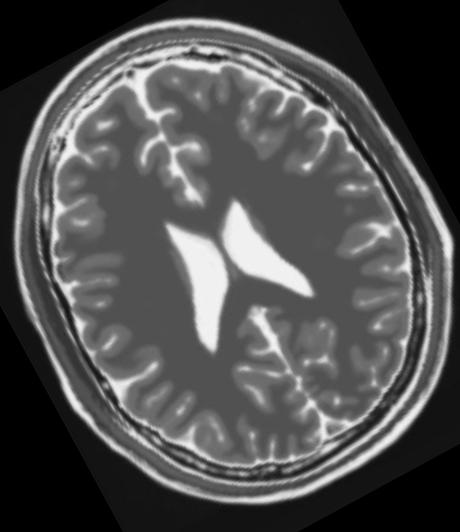
\includegraphics[scale=0.3]{./Q5/J3.jpg}
\caption{Rotated Image J3}
\end{figure}

\newpage
\subsection*{(b)}

The MATLAB code for this question is as follows:
\begin{lstlisting}[frame=single,numbers=left,style=Matlab-Pyglike,breaklines=true,postbreak=\mbox{\textcolor{red}{$\hookrightarrow$}\space}]
angles = -45:1:45;

ncc = zeros(size(angles));
je = ncc;
qmi = ncc;

for i = 1:length(angles)
    J4 = imrotate(J3, angles(i), 'bilinear', 'crop');
    J4(isnan(J4)) = 0;
    
    normJ4 = (J4 - mean(J4(:))) / std(J4(:));
    normJ1 = (J1 - mean(J1(:))) / std(J1(:));
    
    ncc(i) = sum(normJ1(:) .* normJ4(:)) / numel(J1);
    
    jointHist = histcounts2(normJ1(:), normJ4(:), 7); % 256^(1/3) bins approximately
    jointProb = jointHist / sum(jointHist(:));
    je(i) = -sum(jointProb(jointProb > 0) .* log2(jointProb(jointProb > 0)));
    
    P1 = sum(jointProb, 1);
    P2 = sum(jointProb, 2);
    P1P2 = zeros(length(P1));
    for j = 1:length(P1)
        for k = 1:length(P2)
            P1P2(j, k) = P1(j) * P2(k);
        end
    end
    qmi(i) = sum(sum((jointHist - P1P2).^2));
end
\end{lstlisting}

\newpage
\subsection*{(c)}

The plots for the three dependence measures are as follows:
\begin{figure}[H]
\centering
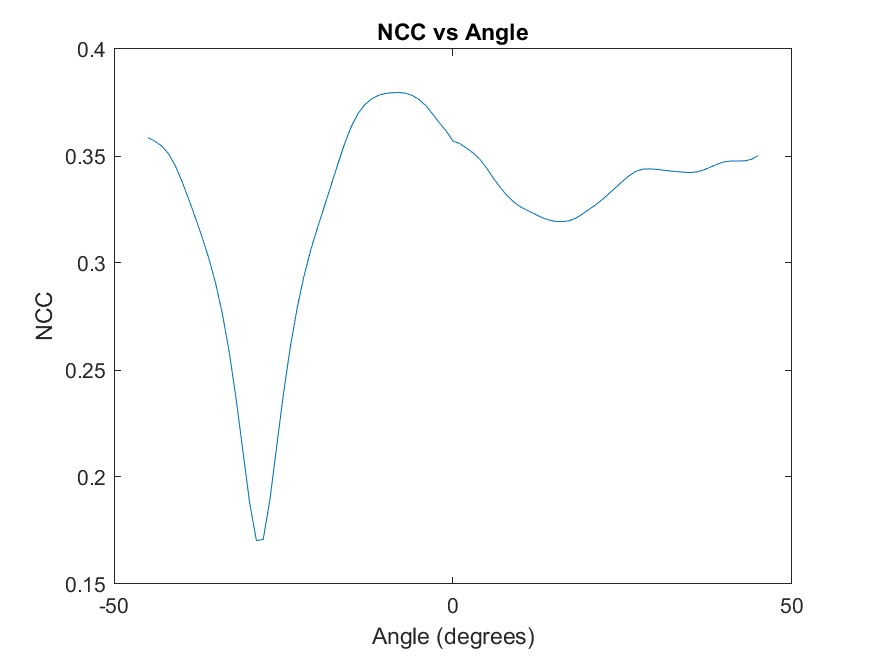
\includegraphics[scale=0.3]{./Q5/NCC_vs_Angle.jpg}
\caption{Normalized Cross Correlation}
\end{figure}

\begin{figure}[H]
\centering
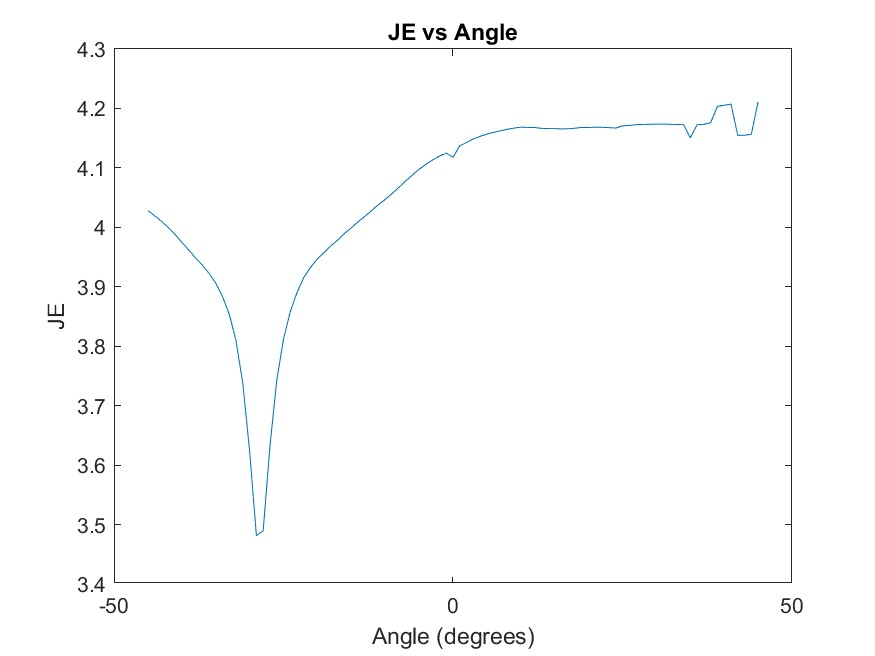
\includegraphics[scale=0.3]{./Q5/JE_vs_Angle.jpg}
\caption{Joint Entropy}
\end{figure}

\begin{figure}[H]
\centering
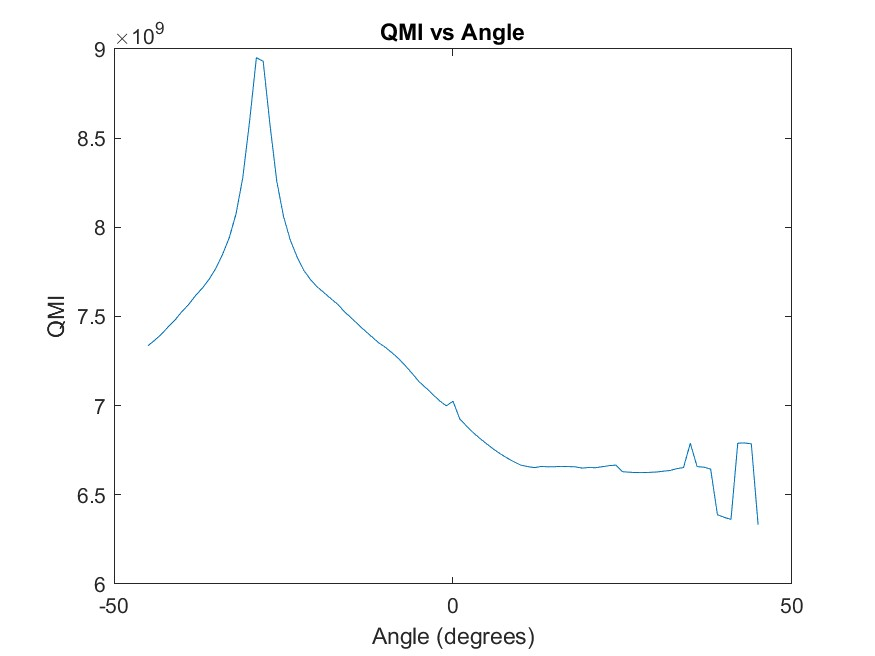
\includegraphics[scale=0.3]{./Q5/QMI_vs_Angle.jpg}
\caption{Quadratic Mutual Information}
\end{figure}

\subsection*{(d)}

The MATLAB code for this question is as follows:
\begin{lstlisting}[frame=single,numbers=left,style=Matlab-Pyglike,breaklines=true,postbreak=\mbox{\textcolor{red}{$\hookrightarrow$}\space}]
[~, nccIndex] = min(ncc);
[~, jeIndex] = min(je);
[~, qmiIndex] = max(qmi);

fprintf('Best NCC angle: %.2f degrees (NCC value: %.4f)\n', angles(nccIndex), ncc(nccIndex));
fprintf('Best JE angle: %.2f degrees (JE value: %.4f)\n', angles(jeIndex), je(jeIndex));
fprintf('Best QMI angle: %.2f degrees (QMI value: %.4f)\n', angles(qmiIndex), qmi(qmiIndex));    
\end{lstlisting}

From the plots, the best angle for the three dependence measures comes out to be \textbf{$29^{\circ}$ counter-clockwise}. We observe that at this angle, the NCC value is minimized, the JE value is minimized and the QMI value is maximized.
Thus all the three dependence measures agree on the best angle of rotation.

\vspace{5pt}
\texttt{Terminal Out:\\Best NCC angle: -29.00 degrees (NCC value: 0.1703)\\
Best JE angle: -29.00 degrees (JE value: 3.4815)\\
Best QMI angle: -29.00 degrees (QMI value: 8951113300.4131)}

\newpage
\subsection*{(e)}

The optimal angle of rotation is $29^{\circ}$ counter-clockwise. The MATLAB code for this question is as follows:
\begin{lstlisting}[frame=single,numbers=left,style=Matlab-Pyglike,breaklines=true,postbreak=\mbox{\textcolor{red}{$\hookrightarrow$}\space}]
optimJ4 = imrotate(J3, angles(jeIndex), 'bilinear', 'crop');
optimJ4(isnan(optimJ4)) = 0;

bins = 37; % 256/7 approximately

histJ1 = histcounts(J1(:), bins);
histJ4 = histcounts(optimJ4(:), bins);

jointHist = zeros(bins);

for i = 1:size(J1, 1)
    for j = 1:size(optimJ4, 2)
        intensity_bin1 = floor(J1(i, j) * (bins - 1)) + 1;
        intensity_bin2 = floor(optimJ4(i, j) * (bins - 1)) + 1;
        jointHist(intensity_bin1, intensity_bin2) = jointHist(intensity_bin1, intensity_bin2) + 1;
    end
end

% Normalize the joint histogram to create a joint probability distribution
jointProb = jointProb / sum(jointHist(:));

% Plot the joint histogram
figure; imagesc(jointProb);
colormap jet;
colorbar;
xlabel('Intensity in J4 (Rotated)');
ylabel('Intensity in J1');
title('Joint Histogram between J1 and J4 (Optimal JE)');
axis xy;
    
% Save the plot as an image
saveas(gcf, 'JointHist_Optimal_JE.jpg');
\end{lstlisting}

The joint histogram between the original image J1 and the optimally rotated image J4 is as follows:
\begin{figure}[H]
\centering
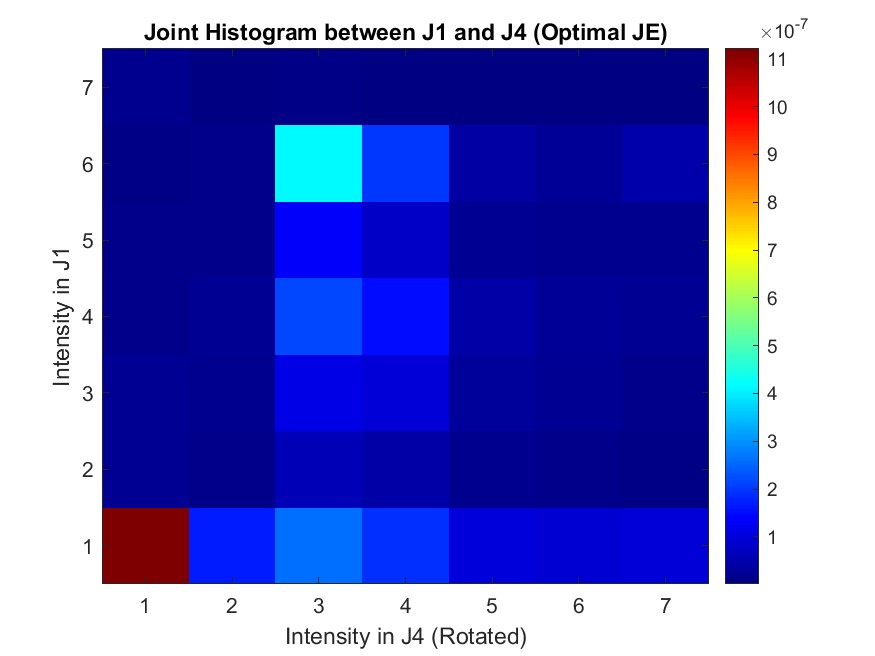
\includegraphics[scale=0.3]{./Q5/JointHist_Optimal_JE.jpg}
\caption{Joint Histogram between J1 and J4 (Optimal JE)}
\end{figure}

\subsection*{(f)}
Quadratic Mutual Information (QMI) measures the statistical relationship between the two random variables, such as pixel intensities in images. It compares the actual joint distribution of these variables to the expected distribution if they were independent.
\vspace{5pt}

If the variables are independent, their joint distribution will be similar to the product of their individual distributions, resulting in a low QMI value. But if the variables are dependent, the joint distribution differs leading to a much higher QMI value.
\vspace{5pt}

Hence, QMI helps identify and quantify the dependence between two variables, capturing details that might not be evident with other measures.

\newpage
\section{Homework 1 - Question 6}

\subsection*{(a)}

The MATLAB code for this question is as follows:
\begin{lstlisting}[frame=single,numbers=left,style=Matlab-Pyglike,breaklines=true,postbreak=\mbox{\textcolor{red}{$\hookrightarrow$}\space}]    
n = 12;
choice = 1; %1 for ginput, else feed directly

if choice == 1
    for i = 1:n
        figure(1); imshow(im1/255); 
        [x1(i),y1(i)] = ginput(1);
        figure(2); imshow(im2/255); 
        [x2(i),y2(i)] = ginput(1);
    end
end

disp("Figure 1 goi1 selected points are:")
disp([x1, y1])
disp("Figure 2 goi2 selected points are:")
disp([x2, y2])
\end{lstlisting}

After running the above code, we get the following selected points for the two images:

\texttt{Terminal Out:\\
Figure 1 goi1 selected points are:\\
   202.3677  512.4066  277.6984  179.0214  316.9202  484.0798  264.9358  118.3210  424.9358  373.8852  367.3482  201.1226  256.7646  294.7412  251.4728  218.4767  219.4105  301.2782  175.8307  246.1809  178.3210   19.5661  210.0720  243.0681
}

\texttt{Figure 2 goi2 selected points are:\\
   236.6089  570.6167  313.8074  212.9514  353.0292  537.3093  299.1770  150.6946  467.2704  414.3521  406.2588  162.5233  277.9319  313.7296  271.0837  238.0875  238.7101  321.5117  192.6401  266.4144  191.3949   32.0175  230.3054  255.2082
}

\subsection*{(b)}

The MATLAB code for this question is as follows:
\begin{lstlisting}[frame=single,numbers=left,style=Matlab-Pyglike,breaklines=true,postbreak=\mbox{\textcolor{red}{$\hookrightarrow$}\space}]
P2 = [x2; y2; ones(1,n)];
P1 = [x1; y1; ones(1,n)];
A = P2*P1'*inv(P1*P1'); % Moore-Penrose pseudo-inverse

disp("Matrix A:")
disp(A);
\end{lstlisting}

After running the above code, we get the following matrix $A$:

\texttt{Terminal Out:\\
Matrix A:\\
\hspace*{2em}1.1047\hspace*{1.5em}-0.0012\hspace*{2.5em}1.2435\\
\hspace*{1.5em}-0.0032\hspace*{2em}1.0283\hspace*{2em}12.6563\\
\hspace*{2em}\hspace*{2.5em}0\hspace*{2em}\hspace*{2.5em}0\hspace*{2em}\hspace*{0.5em}1.0000}

Hence, the image \texttt{goi1} was transformed using the rotation, scaling, shearing and translation transformations to get the image \texttt{goi2}. This can be mathematically achieved using the matrix $A$.

\subsection*{(c)}

The MATLAB code for this question is as follows:
\begin{lstlisting}[frame=single,numbers=left,style=Matlab-Pyglike,breaklines=true,postbreak=\mbox{\textcolor{red}{$\hookrightarrow$}\space}]
im3 = zeros(size(im1));

for i = 1:H 
    for j = 1:W 
        dxy = A\[j i 1]'; 
        xx = round(dxy(1)); 
        yy = round(dxy(2)); 
        
        if xx > 0 && xx <= W && yy > 0 && yy <= H 
            im3(i,j) = im1(yy,xx); % nearest neighbor
        end
    end
end

figure(1); imshow(im1/255);
figure(2); imshow(im2/255);
figure(3); imshow(im3/255);

% Save all the images
saveas(figure(1), 'nn_im1.png');
saveas(figure(2), 'nn_im2.png');
saveas(figure(3), 'nn_im3.png');
\end{lstlisting}

The images obtained after the nearest neighbor interpolation are as follows:
\begin{figure}[htbp]
    \centering
    \begin{minipage}[b]{0.45\textwidth}
        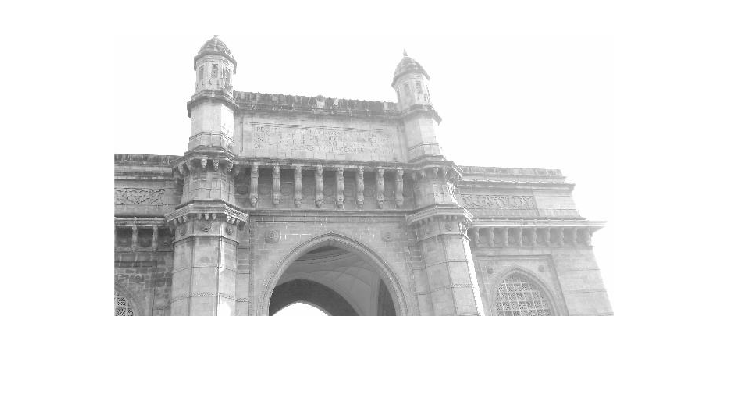
\includegraphics[width=\textwidth]{./Q6/nn_im1.png}
        \caption{\texttt{goi1}}
    \end{minipage}
    % \hfill
    \begin{minipage}[b]{0.45\textwidth}
        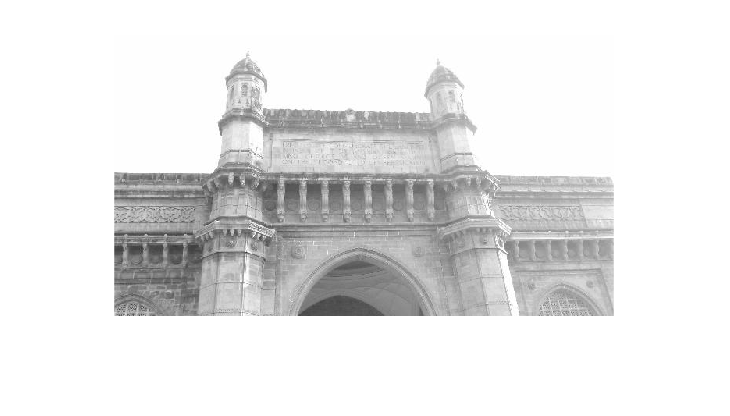
\includegraphics[width=\textwidth]{./Q6/nn_im2.png}
        \caption{\texttt{goi2}}
    \end{minipage}
    % \hfill    
\end{figure}
\begin{figure}[!htb]
    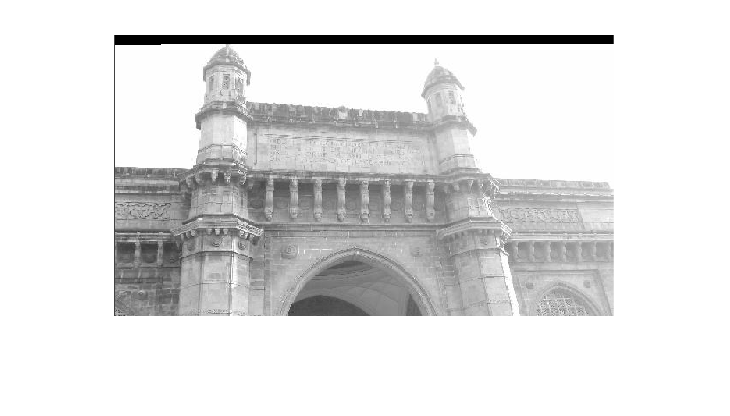
\includegraphics[width=\textwidth]{./Q6/nn_im3.png}
    \caption{Interpolated Image (Nearest Neighbor)}
\end{figure}

\clearpage
\subsection*{(d)}

The MATLAB code for this question is as follows:
\begin{lstlisting}[frame=single,numbers=left,style=Matlab-Pyglike,breaklines=true,postbreak=\mbox{\textcolor{red}{$\hookrightarrow$}\space}]
im4 = zeros(size(im1));

for i = 1:H 
    for j = 1:W 
        dxy = A\[j i 1]'; 
        xx = round(dxy(1)); 
        yy = round(dxy(2)); 
        
        if xx > 0 && xx <= W && yy > 0 && yy <= H 
            w1 = (xx+1-dxy(1))*(yy+1-dxy(2)); % bilinear
            w4 = (dxy(1)-xx)*(dxy(2)-yy);
            w3 = (yy+1-dxy(2))*(dxy(1)-xx);
            w2 = (xx+1-dxy(1))*(dxy(2)-yy);
            im4(i,j) = im1(yy,xx)*w1+im1(yy+1,xx)*w2+im1(yy,xx+1)*w3+im1(yy+1,xx+1)*w4; 
        end
    end
end

figure(1); imshow(im1/255);
figure(2); imshow(im2/255);
figure(3); imshow(im4/255);

% Save all the images
saveas(figure(1), 'bilinear_im1.png');
saveas(figure(2), 'bilinear_im2.png');
saveas(figure(3), 'bilinear_im4.png');
\end{lstlisting}

The images obtained after the bilinear interpolation are as follows:
\begin{figure}[htbp]
    \centering
    \begin{minipage}[b]{0.45\textwidth}
        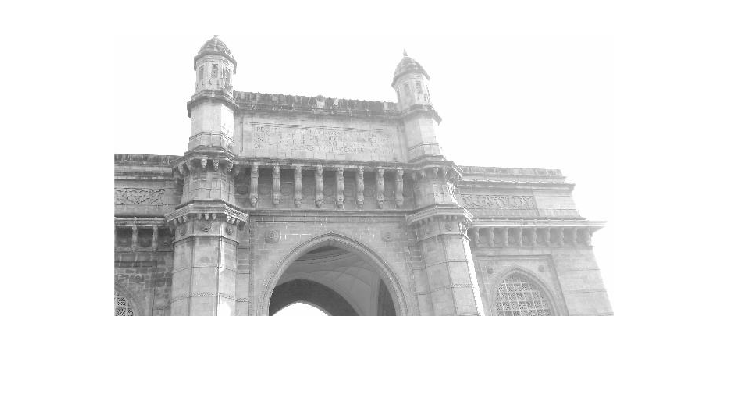
\includegraphics[width=\textwidth]{./Q6/bilinear_im1.png}
        \caption{\texttt{goi1}}
    \end{minipage}
    % \hfill
    \begin{minipage}[b]{0.45\textwidth}
        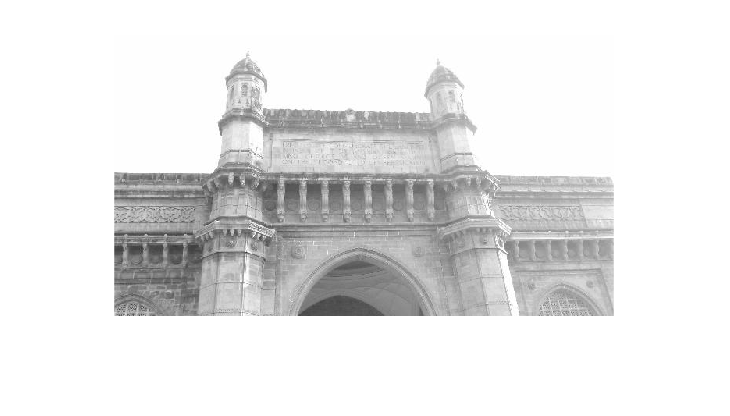
\includegraphics[width=\textwidth]{./Q6/bilinear_im2.png}
        \caption{\texttt{goi2}}
    \end{minipage}
    % \hfill
\end{figure}
\begin{figure}[!htb]
    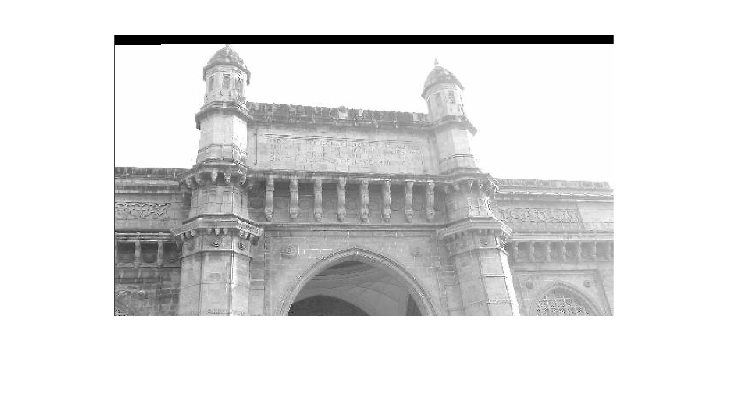
\includegraphics[width=\textwidth]{./Q6/bilinear_im4.png}
    \caption{Interpolated Image (Bilinear)}
\end{figure}

\subsection*{(e)}
For estimating the affine transformation matrix, we need at least three non-collinear points. 

\vspace{5pt}
If all the selected points are collinear, then the following issues may arise:
\begin{enumerate}
\item The system of equations we formed to solve for the affine transformation matrix becomes \textit{underdetermined}, that there is not enough independent equations to uniquely solve for all parameters.
\item The computation will not capture any affine transformation that includes rotations, scaling, or translations.
\item The affine transformation cannot be estimated accurately because the equations would not span the required two-dimensional space. It essentially becomes a problem in one-dimensional space along the line.
\end{enumerate} 


\end{document}